\chapter{Coading}
\section{Introduction of tools and Installation}
\subsection{Android}

There's no other software quite like Android. Google engineered Android, and Google own apps run better on it. And with millions of apps, games, songs, and videos on Google Play, Android is great for fun, and for getting things done.

Android devices come in all kinds of sizes, with all sorts of features, and in all sorts of prices. Each version of Android is named after a dessert, and the most recent version of Android is lolipop. With Android, you’re in control of your mobile experience.

The world is contracting with the growth of mobile phone technology. As the number of users is increasing day by day, facilities are also increasing. Starting with simple regular handsets which were used just for making phone calls, mobiles have changed our lives and have become part of it. Now they are not used just for making calls but they have innumerable uses and can be used as a Camera , Music player, Tablet PC, T.V. , Web browser etc. . And with the new technologies, new software and operating systems are required.


\begin{itemize}
\item What is android
\end{itemize}

{\em Operating Systems} have developed a lot in last 15 years. Starting from black and white phones to recent smart phones or mini computers, mobile OS has come far away. Especially for smart phones, Mobile OS has greatly evolved from Palm OS in 1996 to Windows pocket PC in 2000 then to Blackberry OS and Android. 

\begin{itemize}
\item ADT Bundle
\end{itemize}

The Android SDK is a software development kit which provides API libraries and necessary developer tools necessary for building Android application’s. Android SDK is officially provided by android developers.

{\bfseries steps for the installation and set-up of Android development environment:}
\begin{enumerate}
\item Download Eclipse
\item Download JDK and install it, set the environment path.
\item Download ADT plugin inside Eclipse.
\item Set the Preference with Android-SDK path.
\item Download the latest platform-tools and everything.
\end {enumerate}

{\bfseries The ADT Bundle includes everything you need to begin developing apps:}
\begin{enumerate}
\item Eclipse + ADT plugin
\item Android SDK Tools
\item Android Platform-tools
\item The latest Android platform
\item The latest Android system image for the emulator
\end {enumerate}

Yes there are also possible ways if you want to use existing version of Eclipse or any other IDE.

\begin{itemize}
\item{\bfseries Setting Up the ADT Bundle:}
\end{itemize}


{\bfseries As you have downloaded ADT bundle, follow below steps to setup it:}

\begin{enumerate}
\item Unpack the ZIP file named ``adt bundle osplatform.zip '' and save it to an appropriate location  such as a ``Development'' directory in your home directory.
\item Open the adt bundle osplatform goto eclipse and next directory and launch eclipse.
\end{enumerate}

\subsection {XAMPP Installation Steps}
\begin{enumerate}
\item Download the software from apachefriend website.

Select the Installer option under the Basic Package. You may be taken to a page that presents you with a bunch of different download locations. Just click one of the download buttons, and then save the file to your desktop. Once downloaded, the installer works like most Windows installers.

\item In Internet Explorer, you may get a warning about downloading the file. Click the yellow information bar that appears above the Web page in IE, and choose Download File…

\item Double-click the .exe file you downloaded.

A window opens, asking you to select the language you’d like to use.

If a warning dialog appears click the "Allow" option to install XAMPP.
\item Choose a language from the menu, and then click OK.

A Setup Wizard window appears, ready to step you through the setup process.
\item Click the Next button.

The installer suggests putting the application on your main drive at C, You can pretty much install it anywhere.
\item Click the Next button once again.

The XAMPP Options window appears. In most cases, it’s fine to leave all the window’s checkboxes just as you see.
\item Click Install.

The installer places all the files onto your system. This process takes a while, since a lot of programs and files are being installed.
\item Finally, click the Finish button.

A window appears ``congratulating'' you way to double-click the installer program and asking whether you wish to start the XAMPP Control panel.
\item Click Yes, to open the XAMPP Control Panel .

The XAMPP Control Panel lets you start and stop the Apache Web server and MySQL database server.
\item If the buttons to the right of Apache and MySQL say Start, click them to start the Web server and the MySQL database server.
\item To do so, launch a Web browser, and, in the Location bar and type localhost.

\end{enumerate}


\subsection{PHP}
PHP (recursive acronym for {\bf PHP:} {\em Hypertext Preprocessor}) is a widely-used open source general-purpose scripting language that is especially suited for web development and can be embedded into HTML.

PHP is probably the most popular scripting language on the web. It is used to enhance web pages. With PHP, you can do things like create a username and password login pages, check details from a form, create forums, picture galleries, surveys, and a whole lot more.
 
PHP is known as a server-sided language. That's because the PHP doesn't get executed on your computer, but on the computer you requested the page from. The results are then handed over to you. 

The most popular explanation of just what PHP stands for is "Hypertext Pre-processor". But that would make it HPP, surely? An alternative explanation is that the initials come from the earliest version of the program, which was called Personal Home Page Tools. At least you get the letters "PHP" in the right order!
\begin{itemize}

\item {\bfseries What is a PHP File}
\begin{itemize}

\item PHP files can contain text, HTML, CSS, JavaScript, and PHP code
\item PHP code is executed on the server, and the result is returned to the browser as plain HTML
\item PHP files have extension ". PHP"
\end{itemize}

\item {\bfseries What Can PHP Do}
\begin{itemize}

\item PHP can generate dynamic page content
\item PHP can create, open, read, write, and close files on the server
\item PHP can send and receive cookies
\item PHP can add, delete, modify data in your database.
\item With PHP you are not limited to output HTML. You can output images, PDF files, and even flash movies. You can also output any text, such as XHTML and XML.
\end{itemize}

\item {\bfseries Why PHP}

\begin{itemize}
\item PHP runs on various platforms like Windows, Linux, Unix, Mac OS X, etc.
\item PHP is compatible with almost all servers used today Apache, Apache Tomcat,IIS, etc.
\item PHP supports a wide range of databases
\item PHP is free. Download it from the official PHP resource website.
\end{itemize}
\end{itemize}


\subsection{MySQL}
MySQL, the most popular Open Source SQL database management system, is developed, distributed, and supported by Oracle Corporation.
The MySQL official web site www.mysql.com provides the latest information about MySQL software.
\begin{itemize}
\item MySQL is a database management system.

A database is a structured collection of data. It may be anything from a simple shopping list to a picture gallery or the vast amounts of information in a corporate network. To add, access, and process data stored in a computer database, you need a database management system such as MySQL Server. Since computers are very good at handling large amounts of data, database management systems play a central role in computing, as standalone utilities, or as parts of other applications.

\item MySQL databases are relational.

A relational database stores data in separate tables rather than putting all the data in one big storeroom. The database structures are organized into physical files optimized for speed. The logical model, with objects such as databases, tables, views, rows, and columns, offers a flexible programming environment. You set up rules governing the relationships between different data fields, such as one-to-one, one-to-many, unique, required or optional, and “pointers” between different tables. The database enforces these rules, so that with a well-designed database, your application never sees inconsistent, duplicate, orphan, out-of-date, or missing data.
The SQL part of ``MySQL'' stands for ``Structured Query Language''. SQL is the most common standardized language used to access databases. Depending on your programming environment, you might enter SQL directly for example, to generate reports, embed SQL statements into code written in another language, or use a language-specific API that hides the SQL syntax.


\item MySQL software is Open Source.

Open Source means that it is possible for anyone to use and modify the software. Anybody can download the MySQL software from the Internet and use it without paying anything. If you wish, you may study the source code and change it to suit your needs. The MySQL software uses the GPL for GNU General Public License, to define what you may and may not do with the software in different situations.

\item The MySQL Database Server is fast, reliable, scalable and easy to use.

MySQL Server can run comfortably on a desktop or laptop, alongside your other applications, web servers, and so on, requiring little or no attention. If you dedicate an entire machine to MySQL, you can adjust the settings to take advantage of all the memory, CPU power, and IO capacity available. MySQL can also scale up to clusters of machines, networked together.
MySQL Server was originally developed to handle large databases much faster than existing solutions and has been successfully used in highly demanding production environments for several years. Although under constant development, MySQL Server today offers a rich and useful set of functions. Its connectivity, speed, and security make MySQL Server highly suited for accessing databases on the Internet.
\end{itemize}




\section{Snippets}



\begin{figure}[h!]

\centering
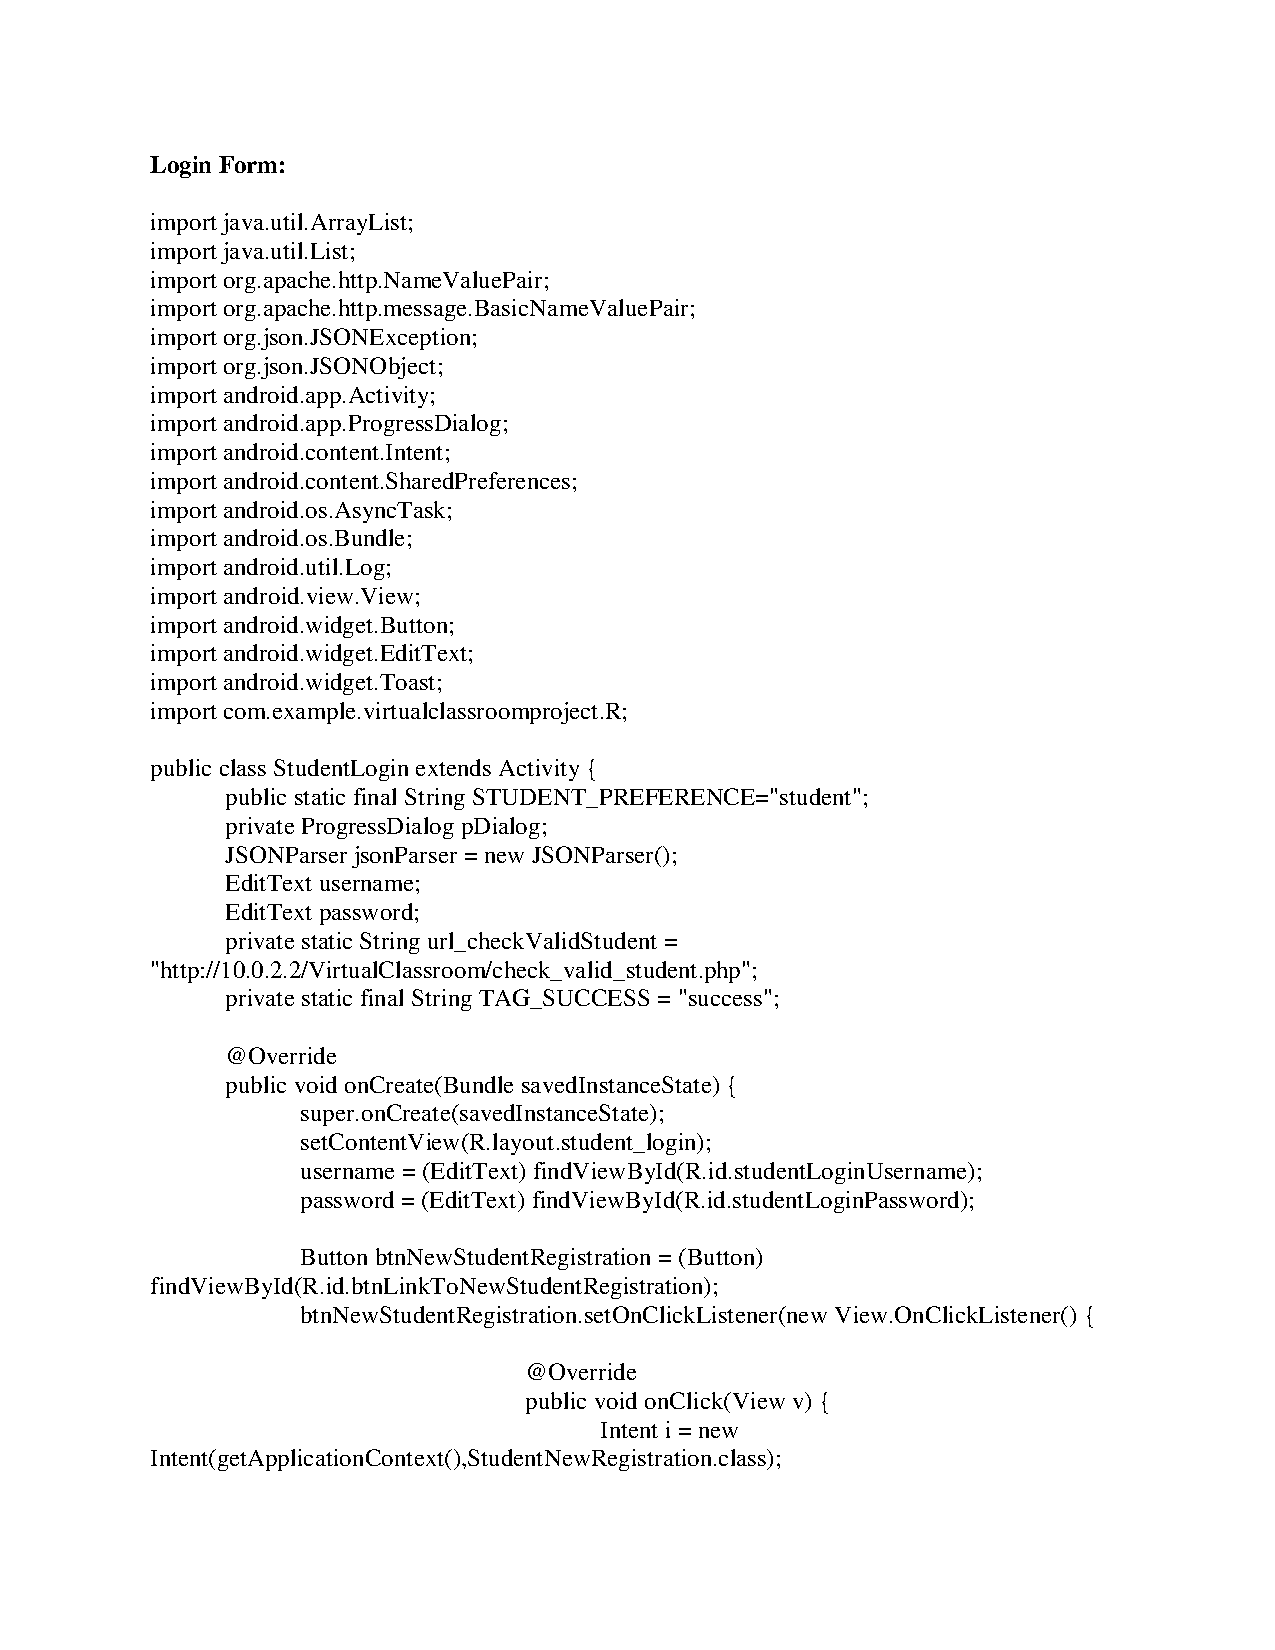
\includegraphics[width=6in]
{code.pdf}
%caption{snapshots}
\end{figure}



\begin{figure}[h!]
\centering
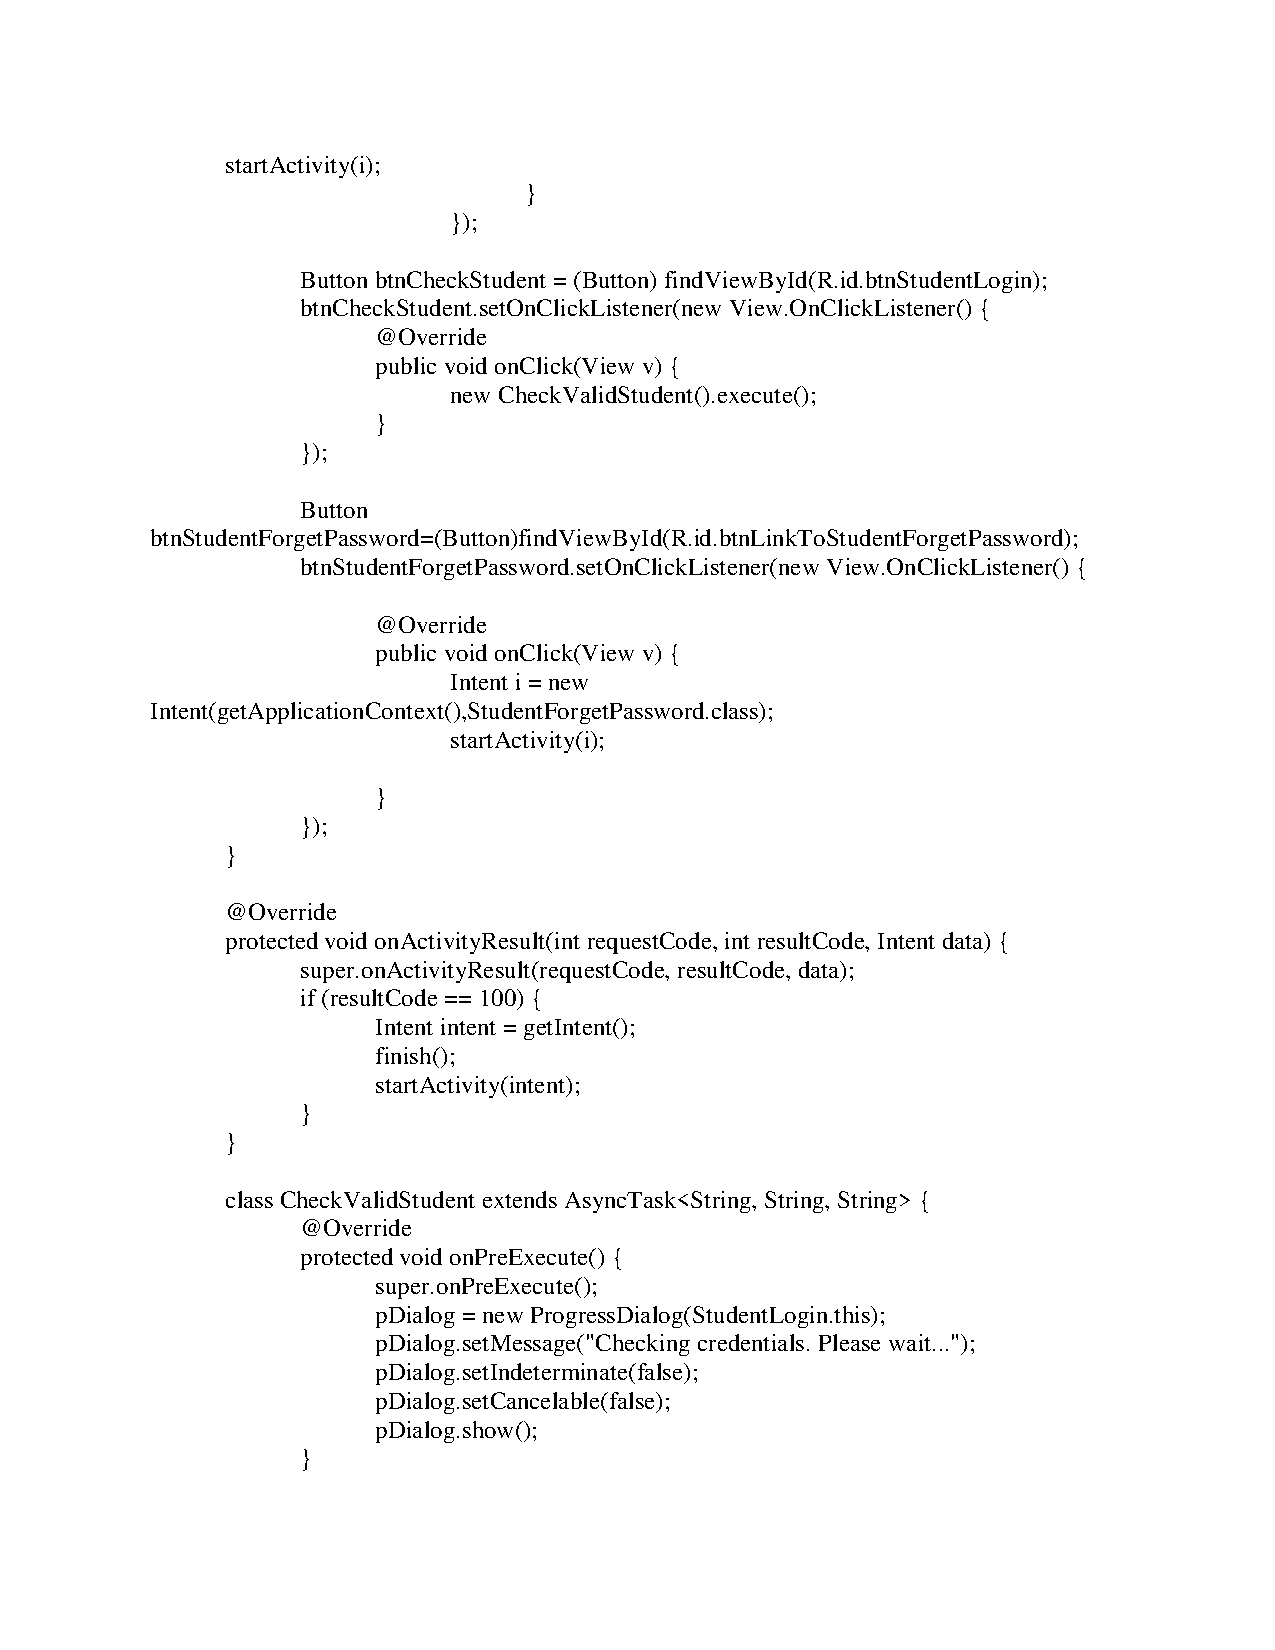
\includegraphics[width=6in]
{code1.pdf}
%\caption{snapshots}
\end{figure}

\begin{figure}[h!]
\centering
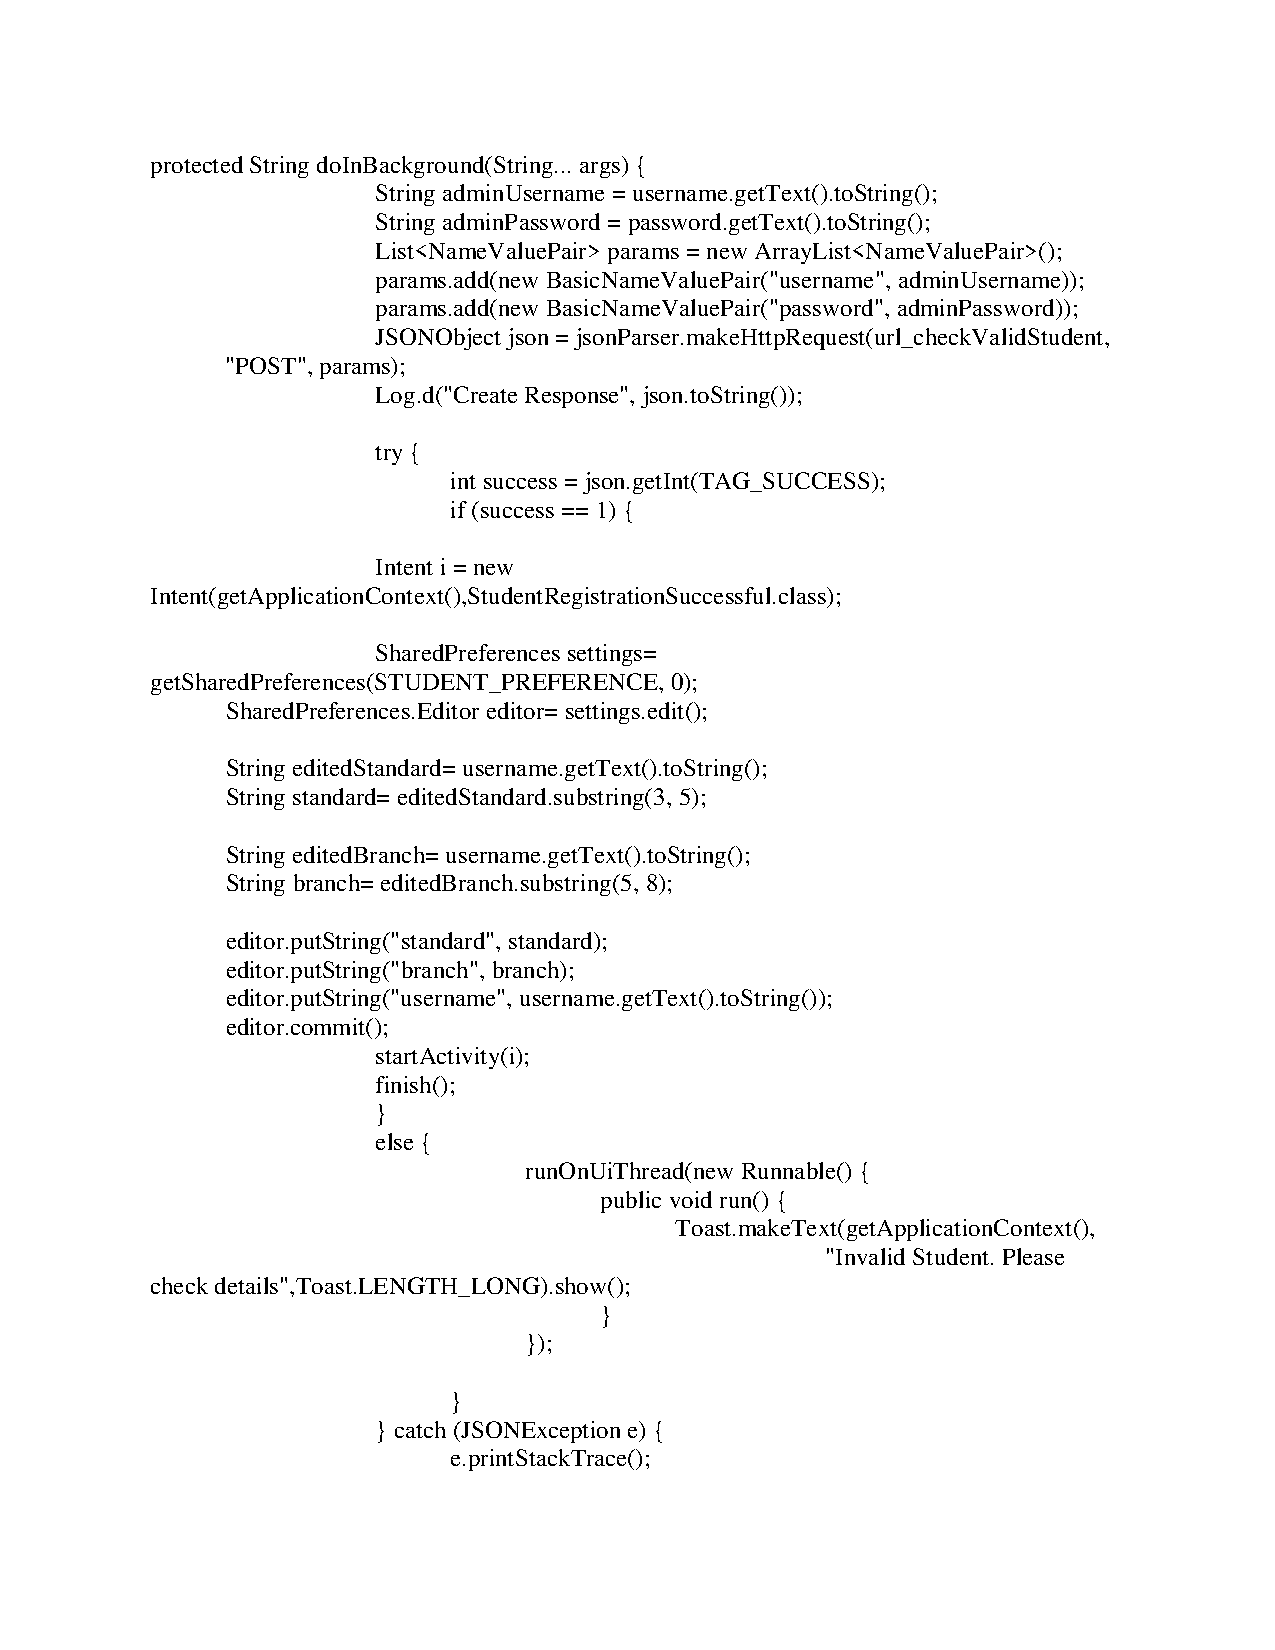
\includegraphics[width=6in]
{code2.pdf}
%\caption{snapshots}
\end{figure}


\begin{figure}[h!]
\centering
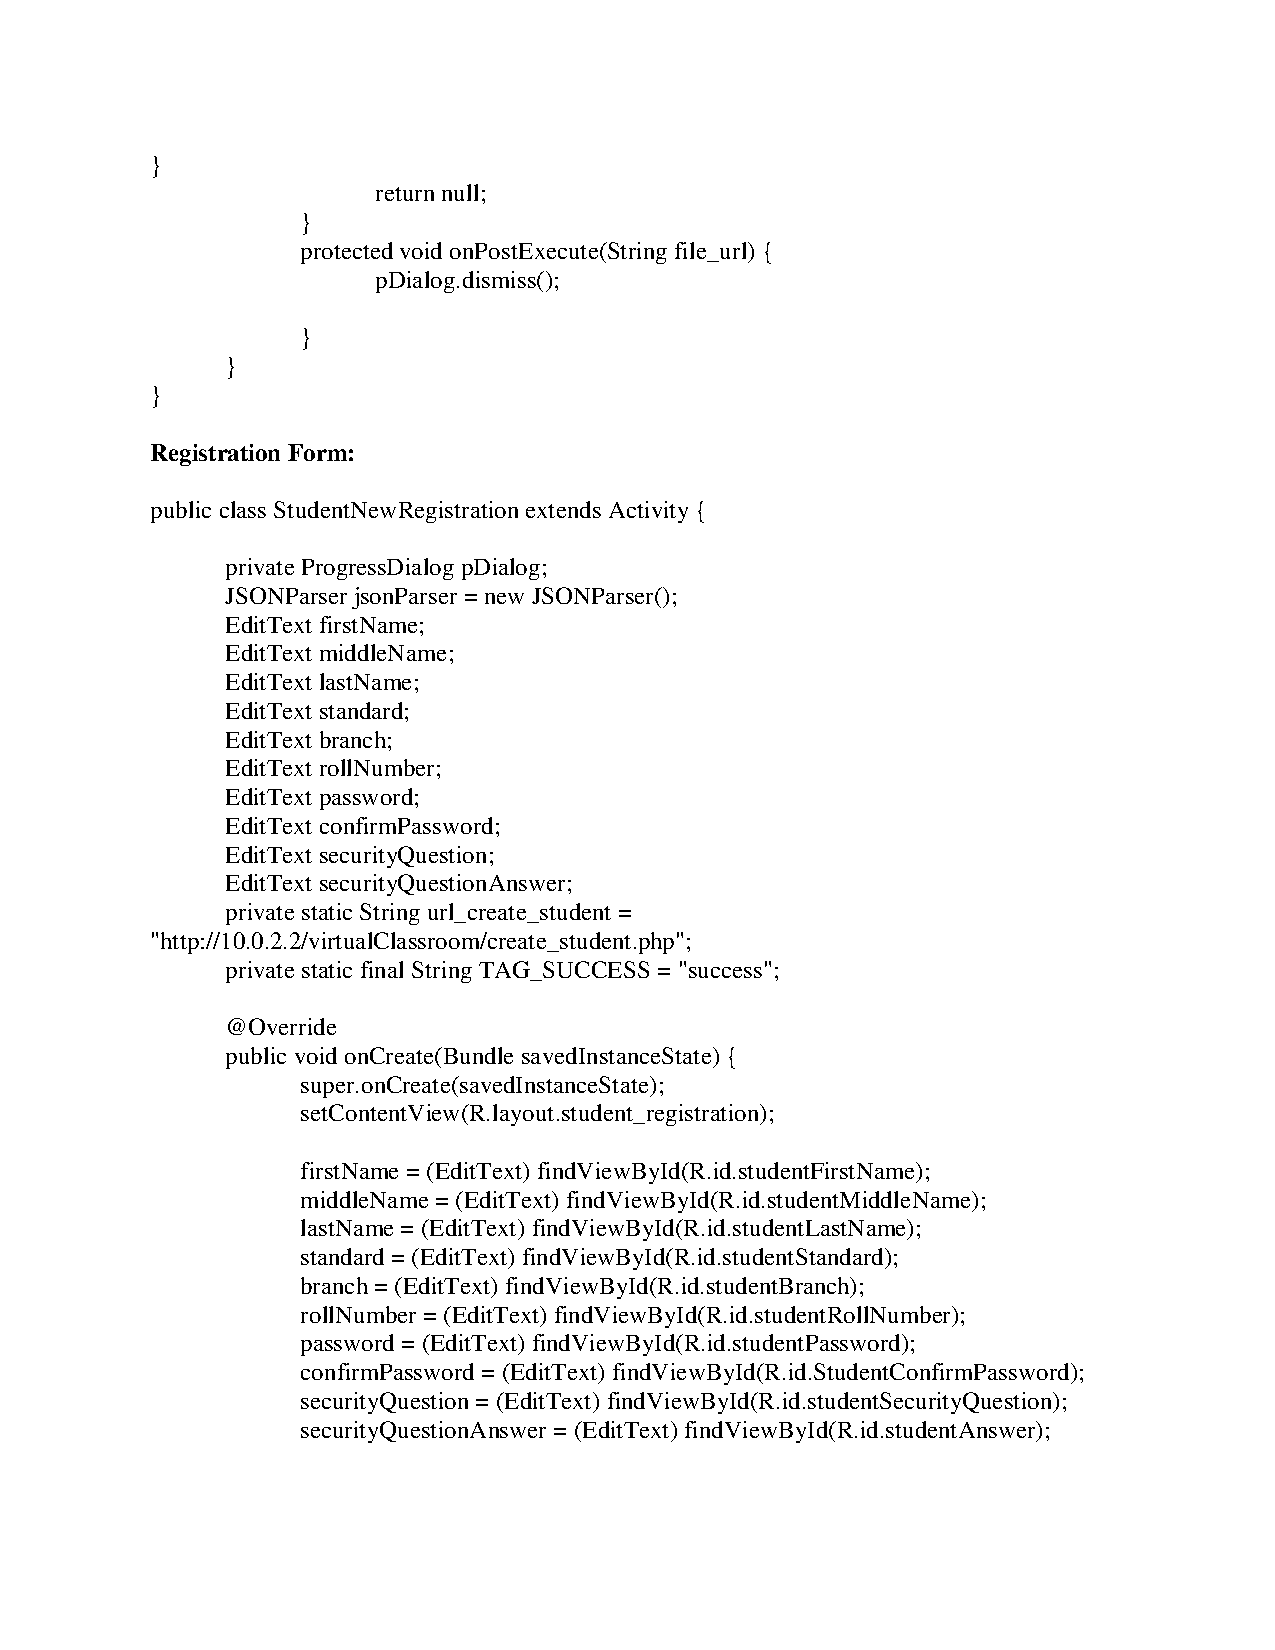
\includegraphics[width=6in]
{code3.pdf}
%\caption{snapshots}
\end{figure}

\begin{figure}[h!]
\centering
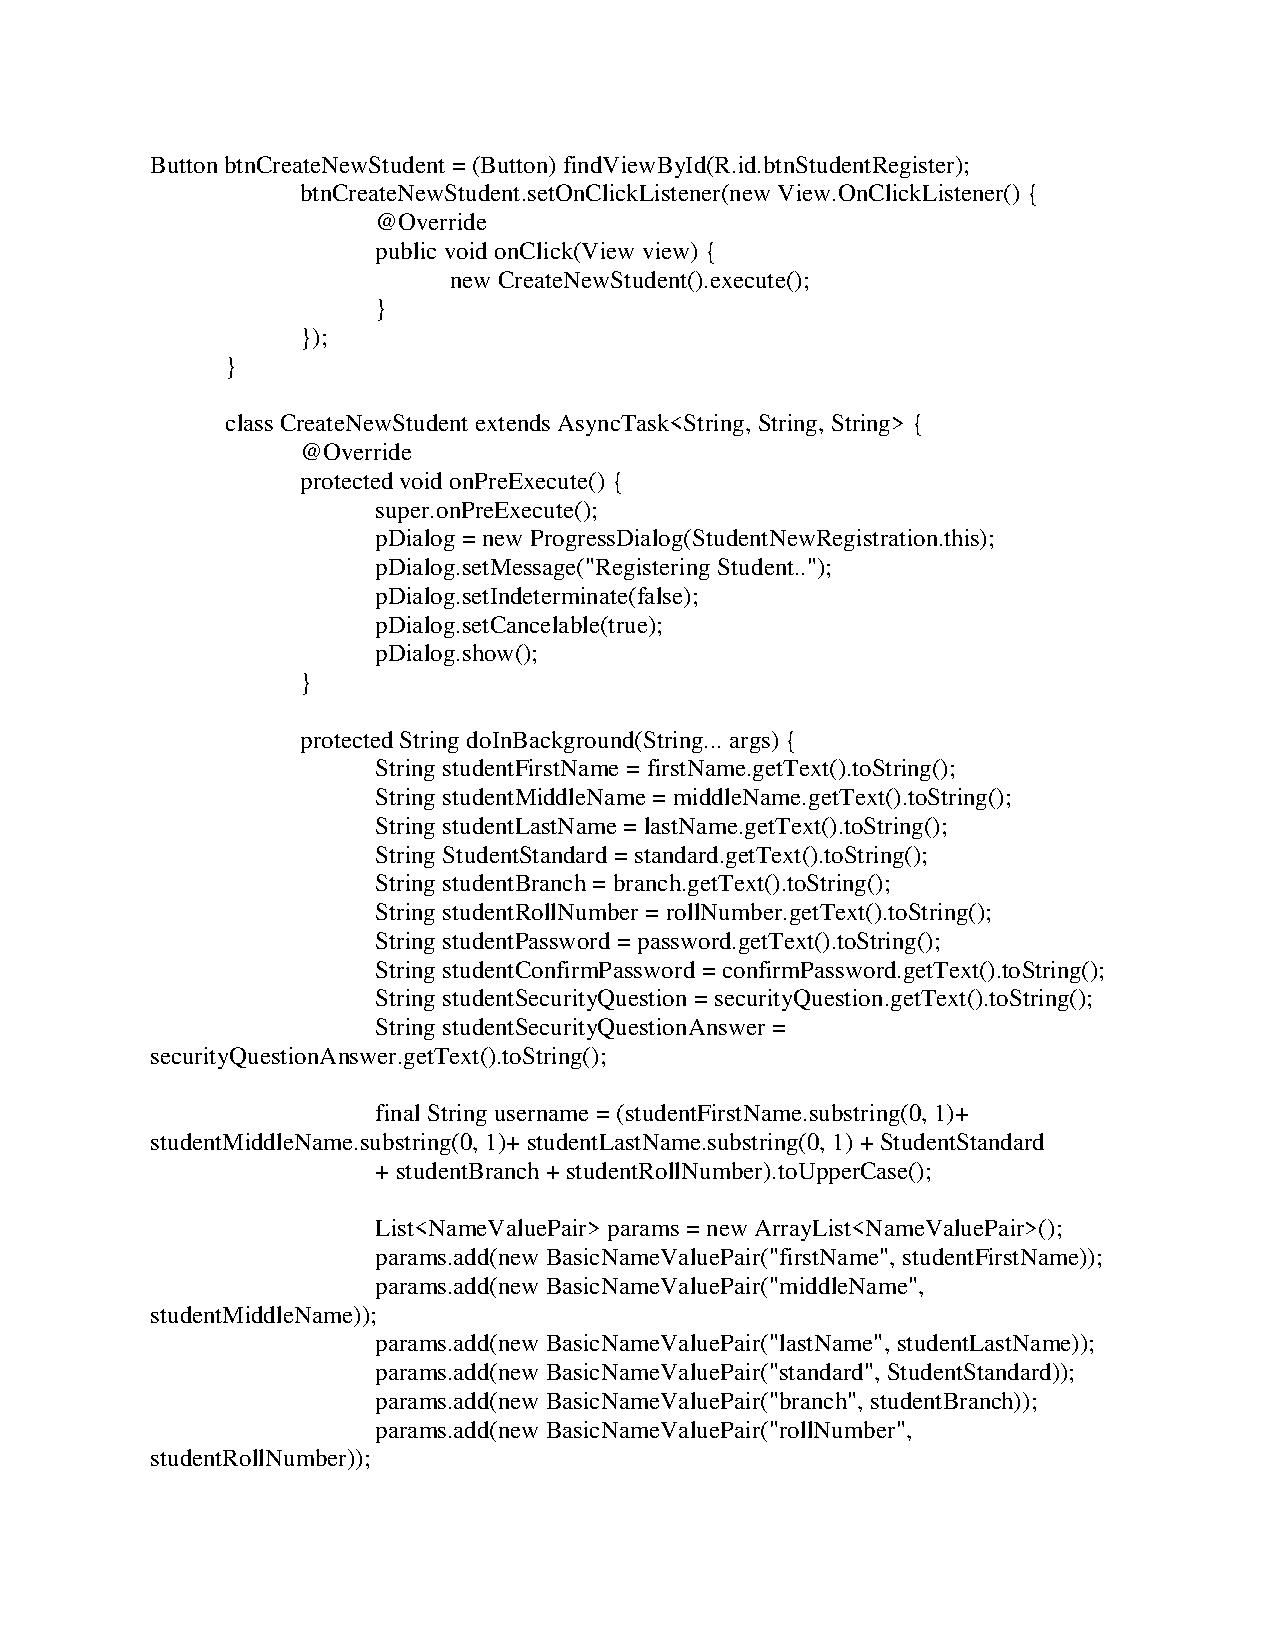
\includegraphics[width=6in]
{code4.pdf}
%\caption{snapshots}
\end{figure}

\begin{figure}[h!]
\centering
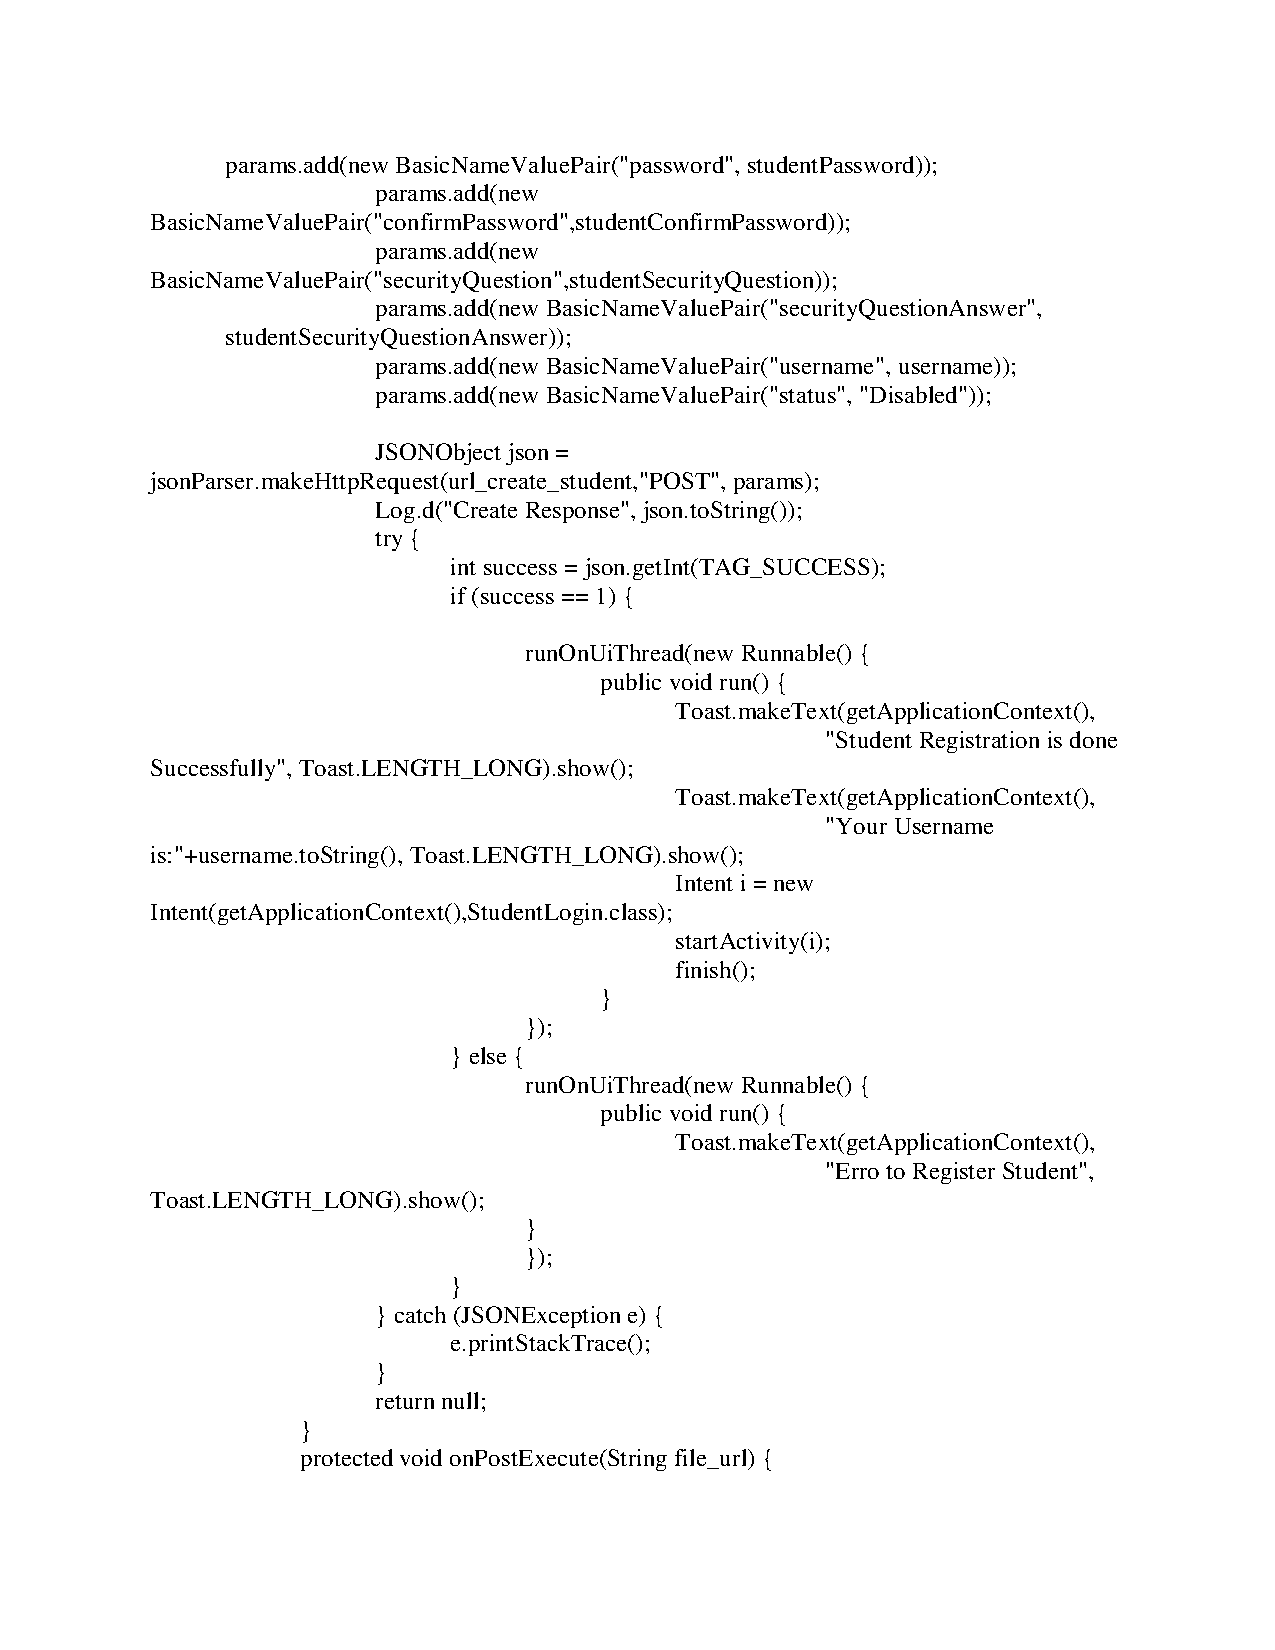
\includegraphics[width=6in]
{code5.pdf}
%\caption{snapshots}
\end{figure}

\begin{figure}[h!]
\centering
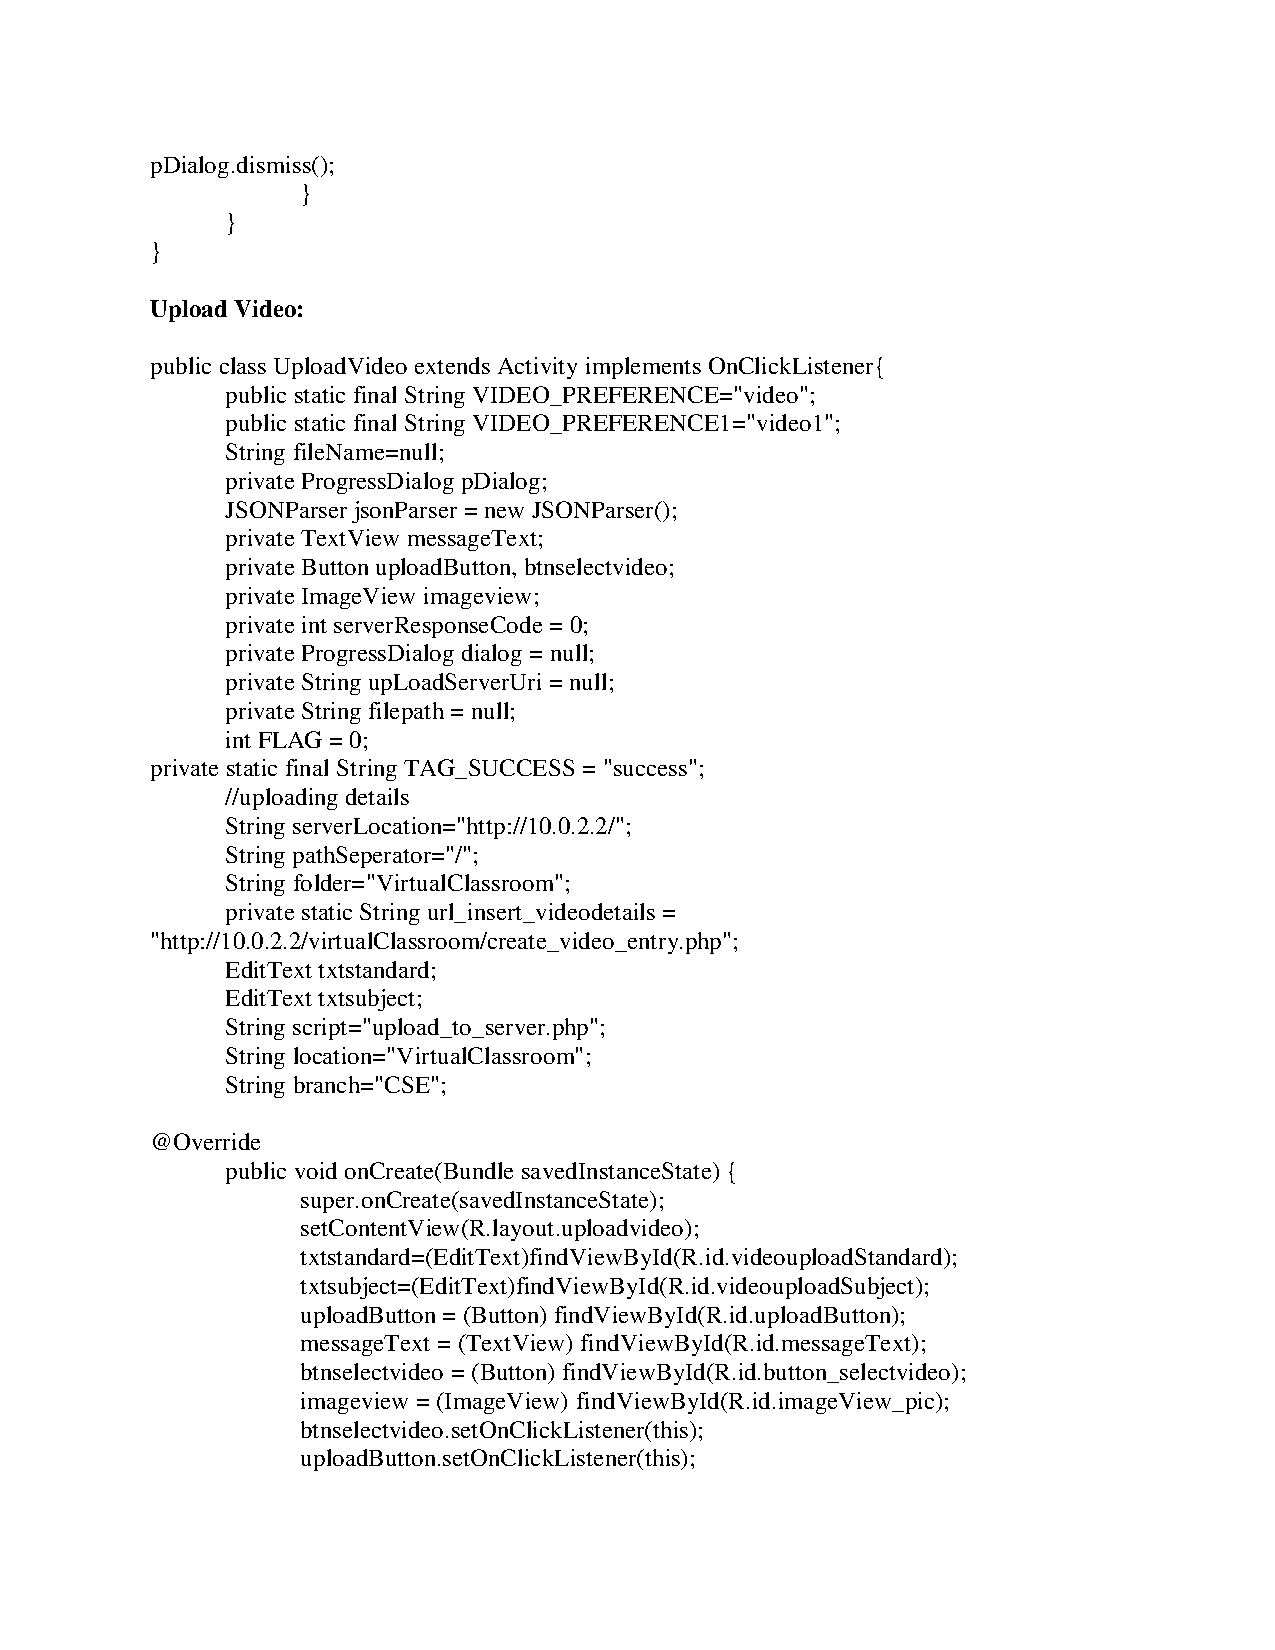
\includegraphics[width=6in]
{code6.pdf}
%\caption{snapshots}
\end{figure}

\begin{figure}[h!]
\centering
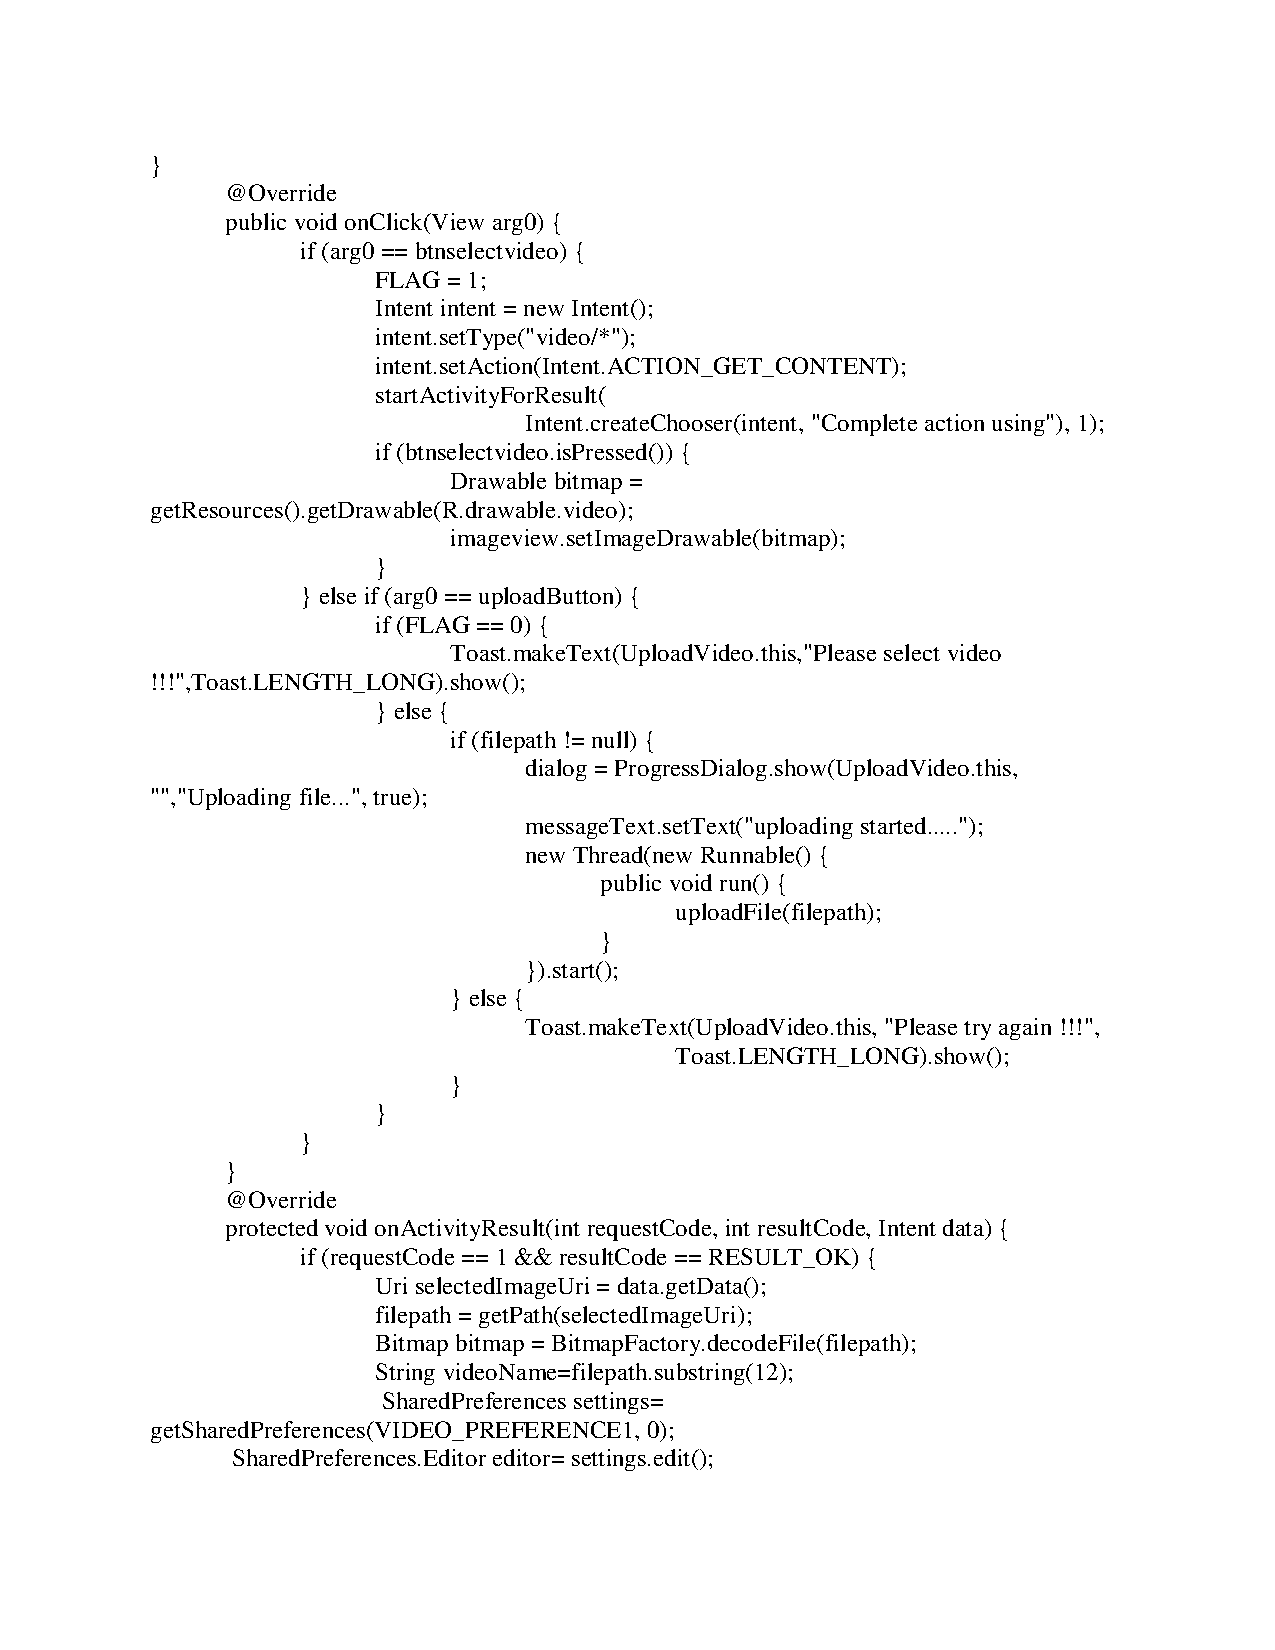
\includegraphics[width=6in]
{code7.pdf}
%\caption{snapshots}
\end{figure}

\begin{figure}[h!]
\centering
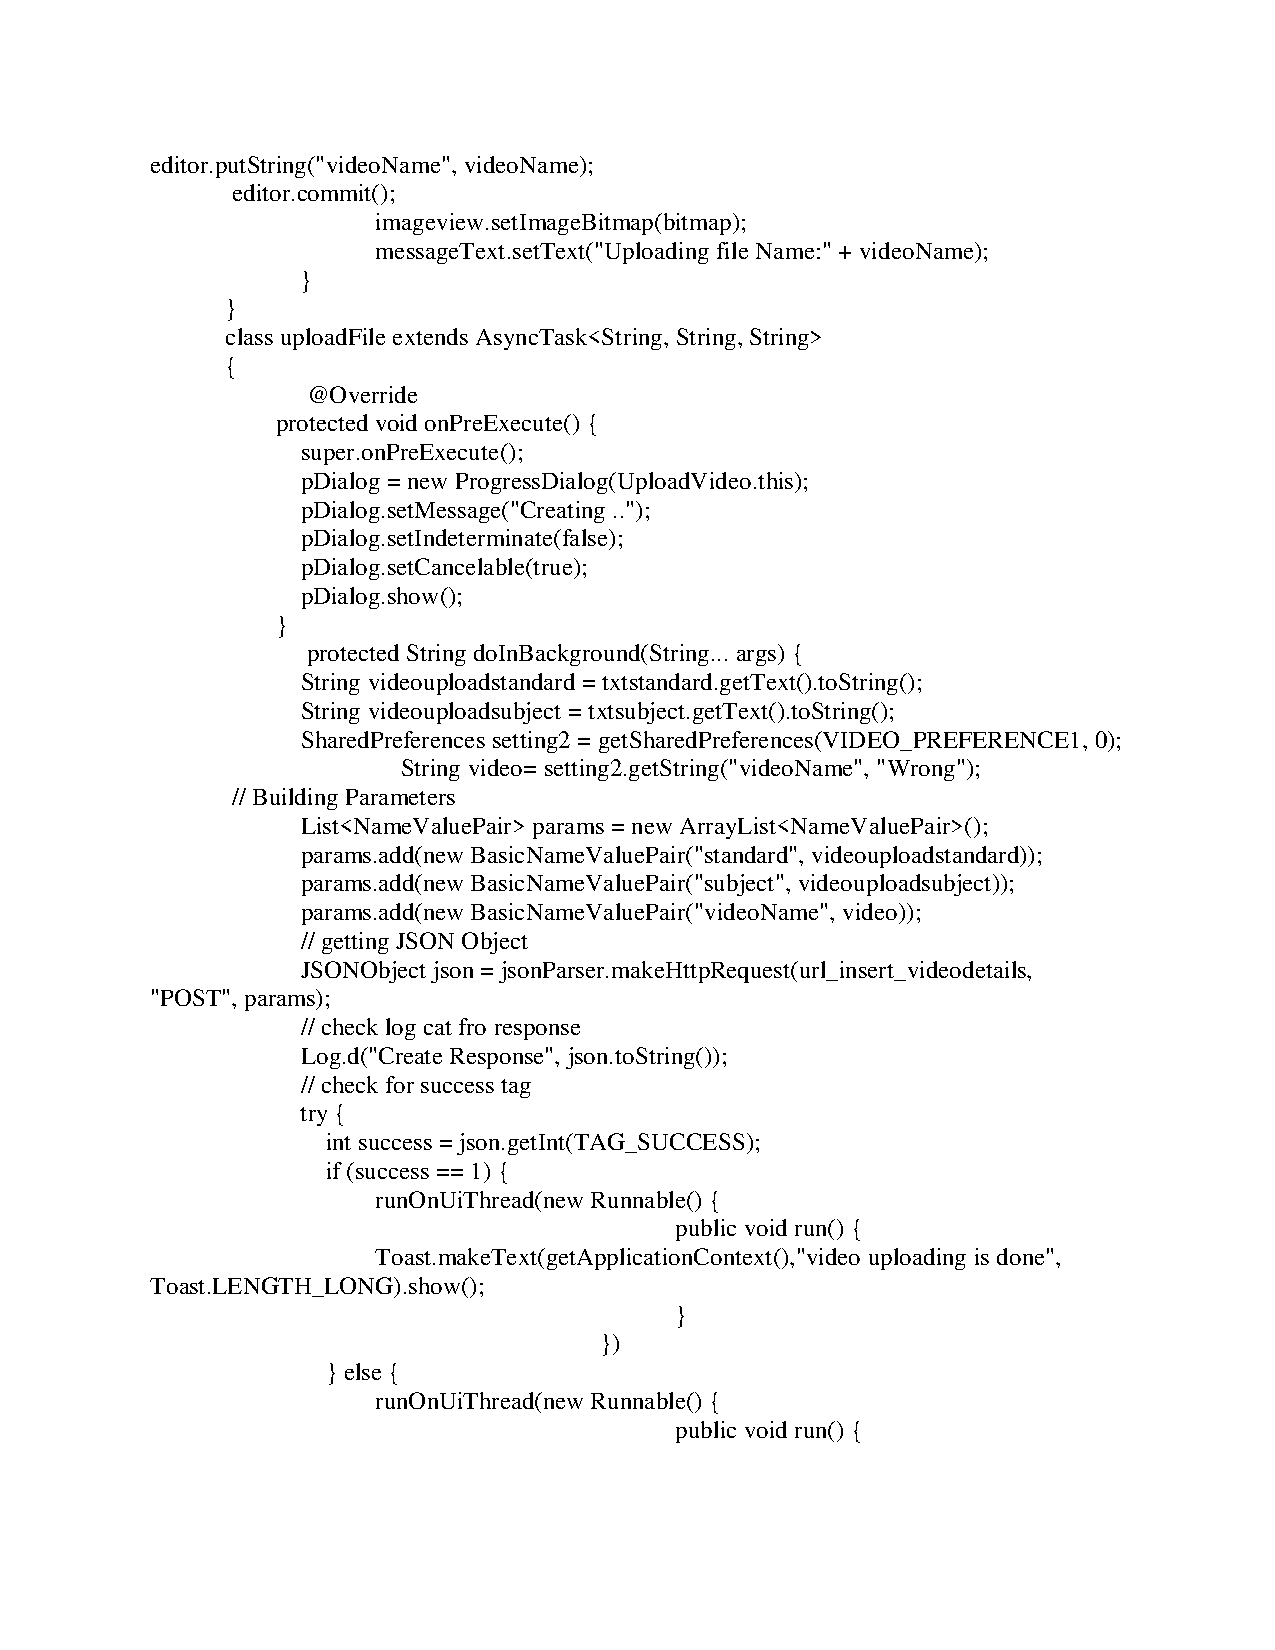
\includegraphics[width=6in]
{code8.pdf}
%\caption{snapshots}
\end{figure}

\begin{figure}[h!]
\centering
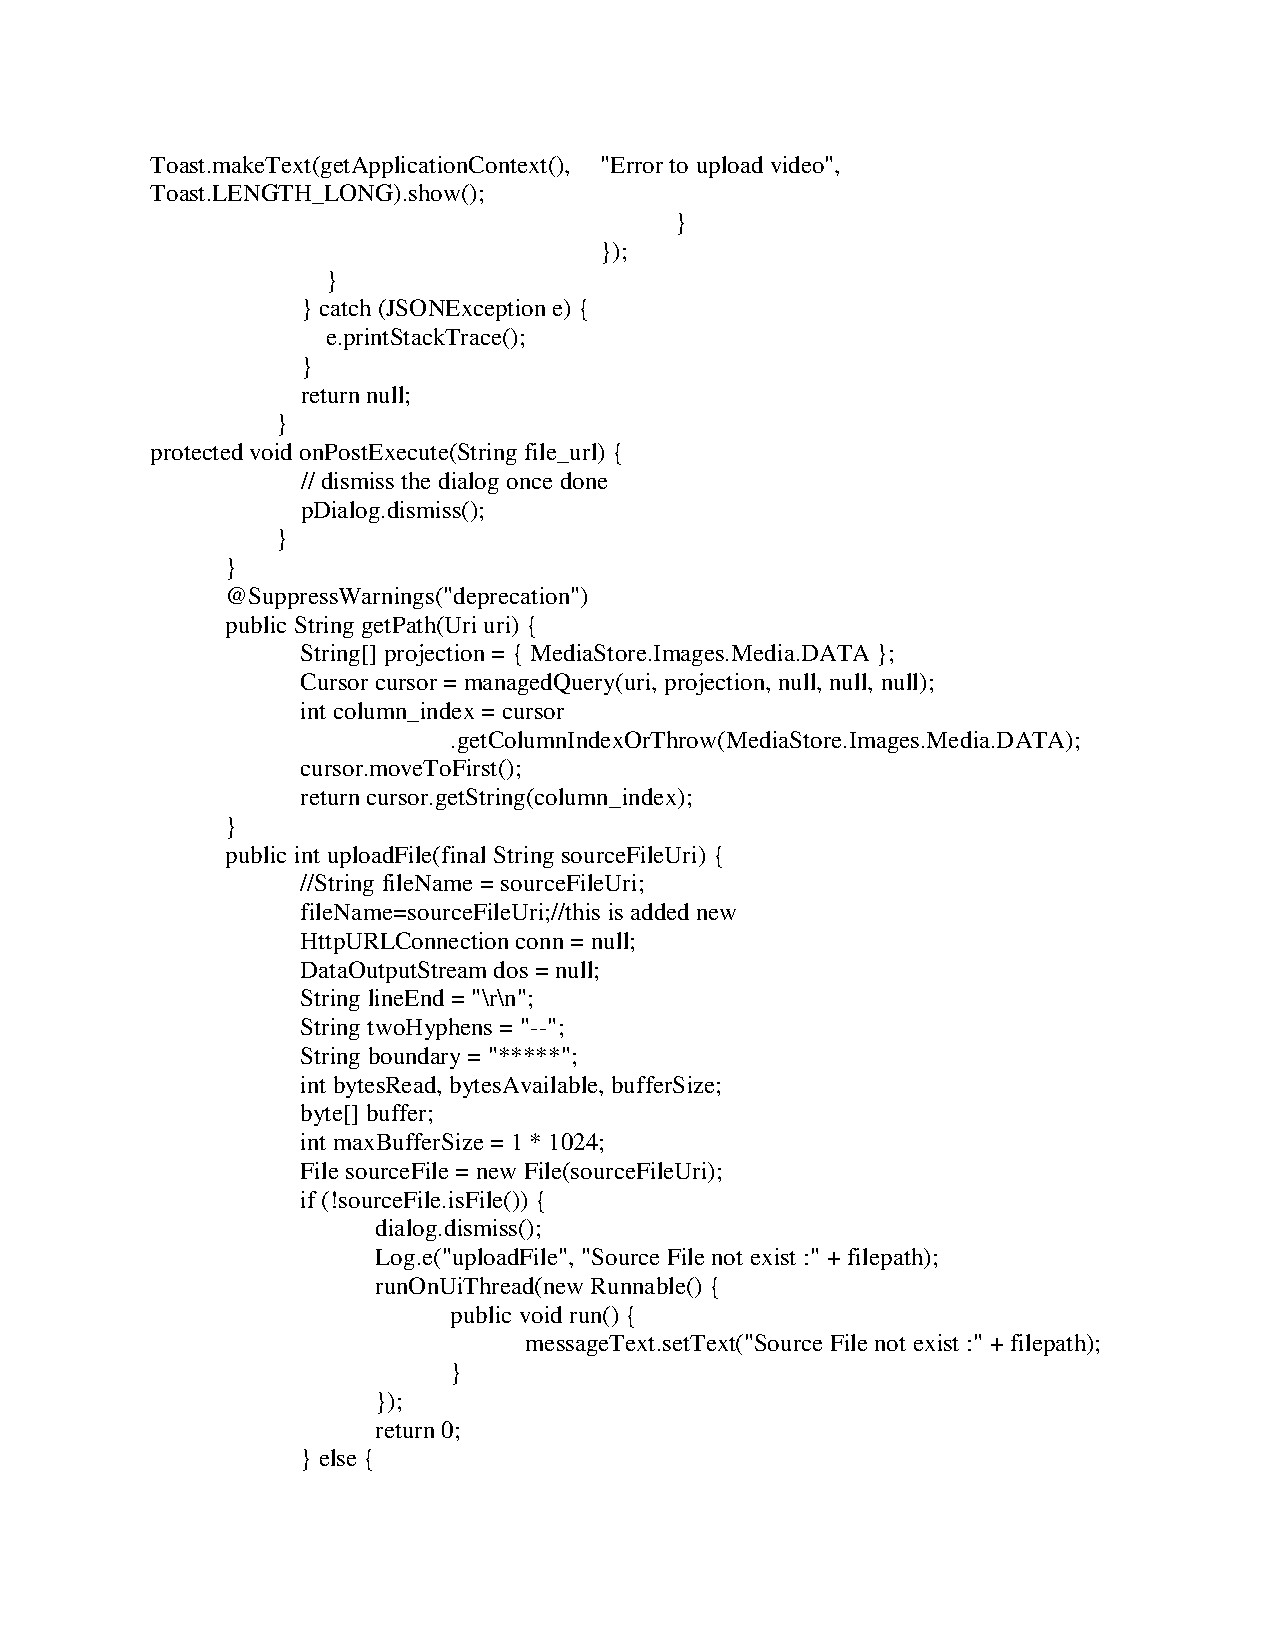
\includegraphics[width=6in]
{code10.pdf}
%\caption{snapshots}
\end{figure}

\begin{figure}[h!]
\centering
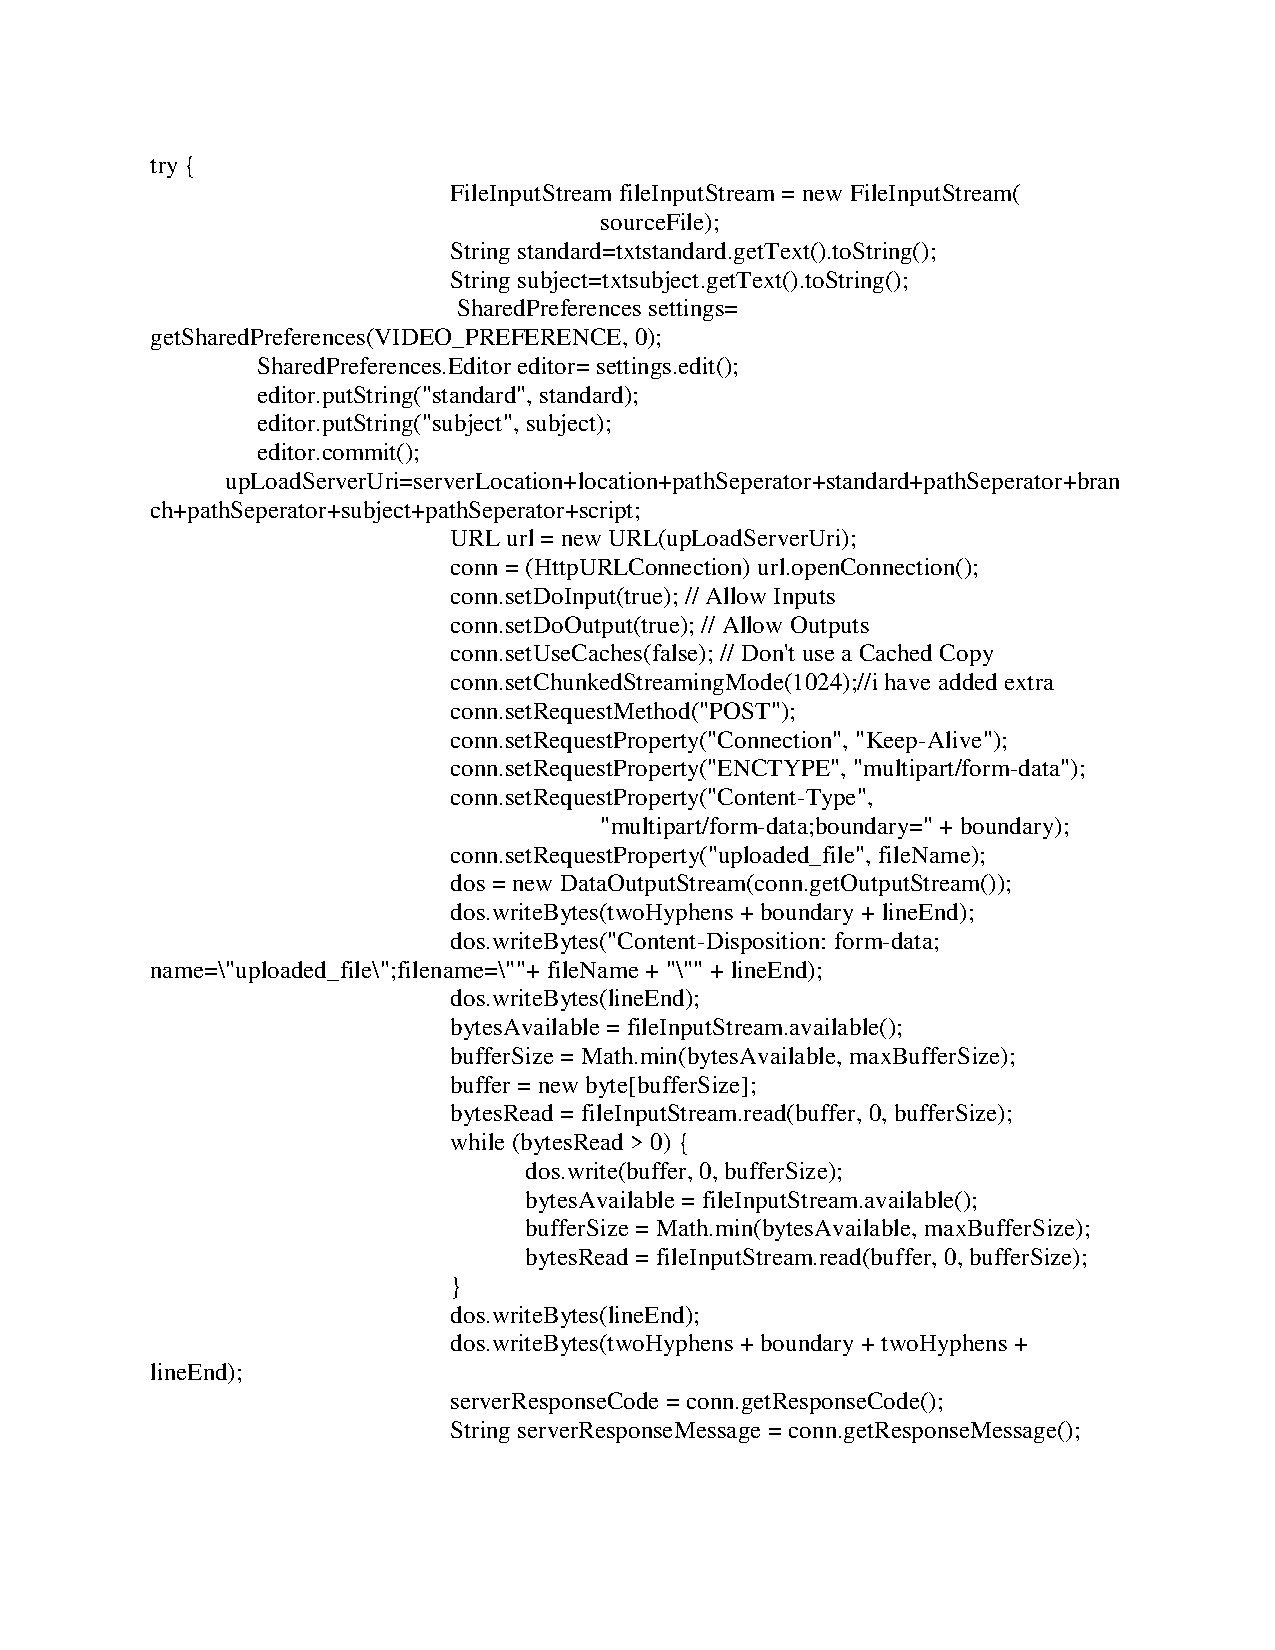
\includegraphics[width=6in]
{code11.pdf}
%\caption{snapshots}
\end{figure}

\begin{figure}[h!]
\centering
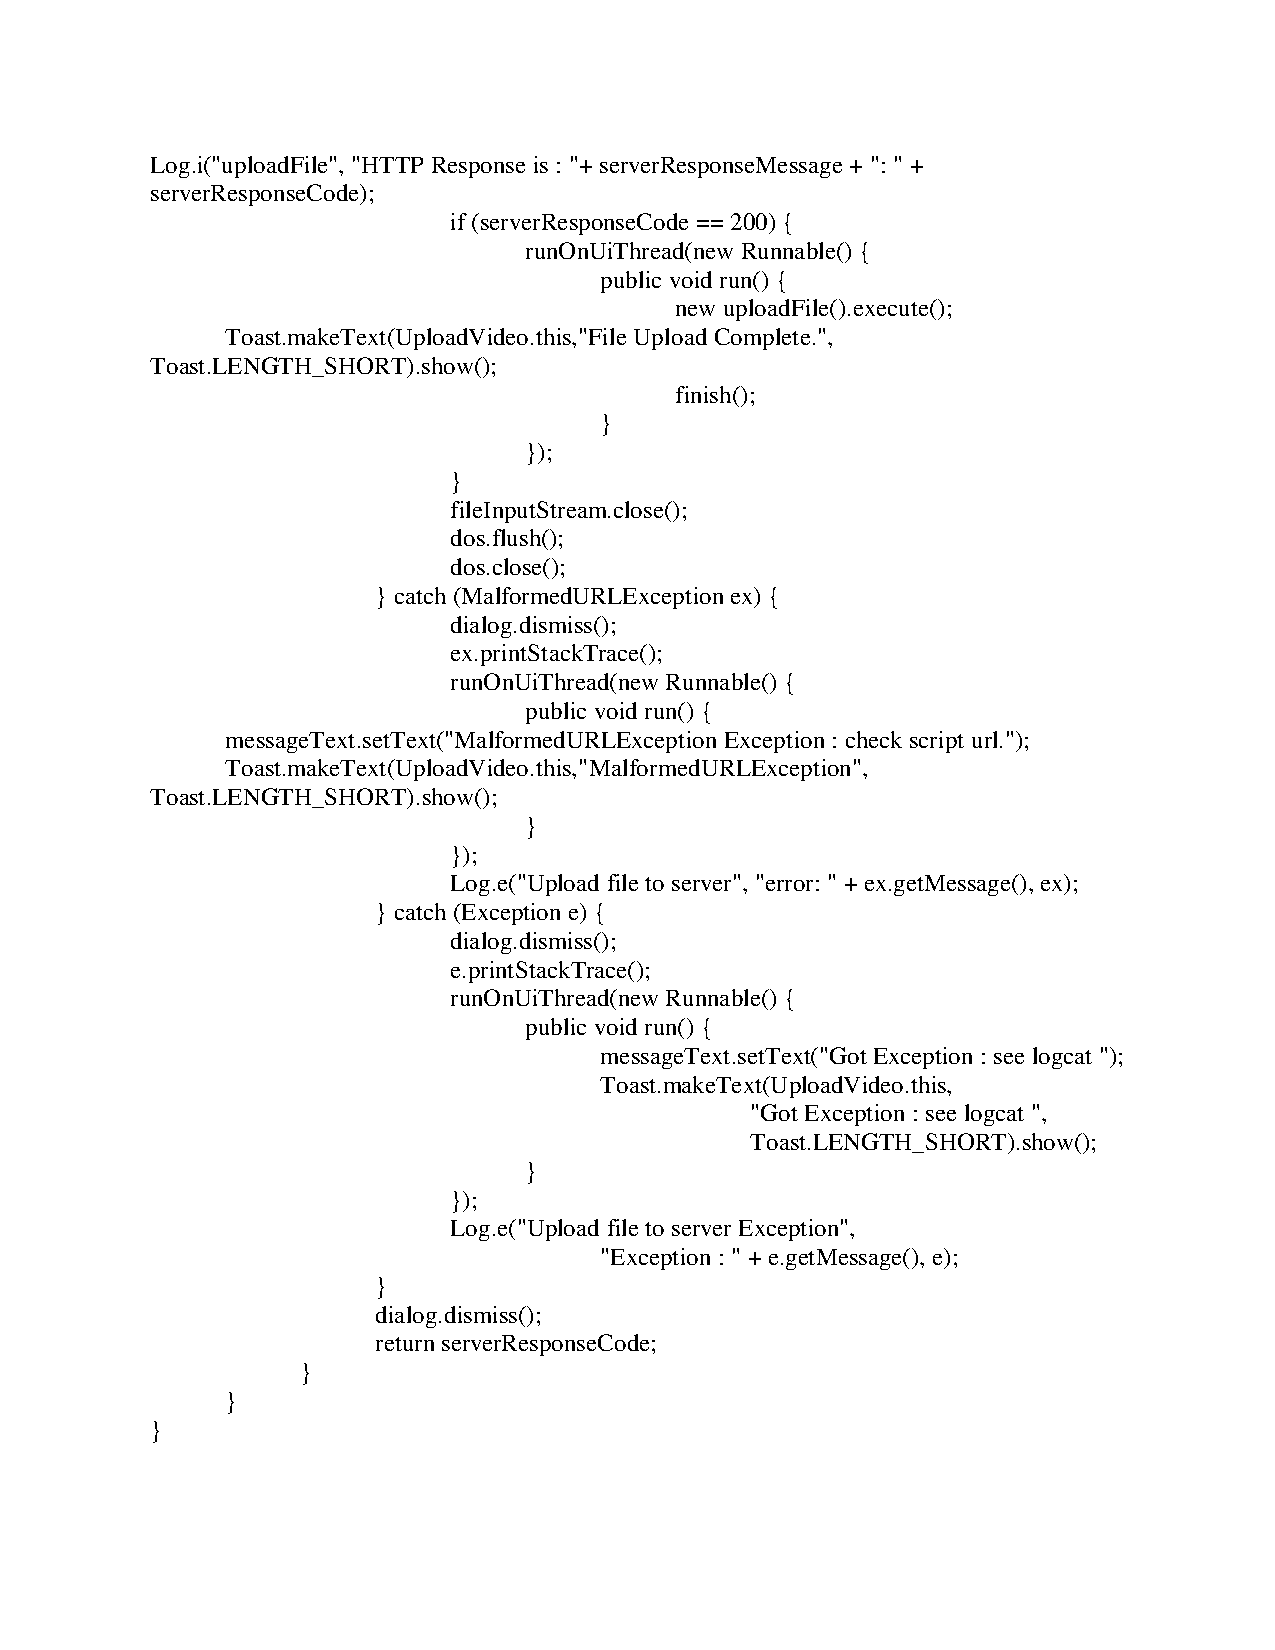
\includegraphics[width=6in]
{code12.pdf}
%\caption{snapshots}
\end{figure}

\begin{figure}[h!]
\centering
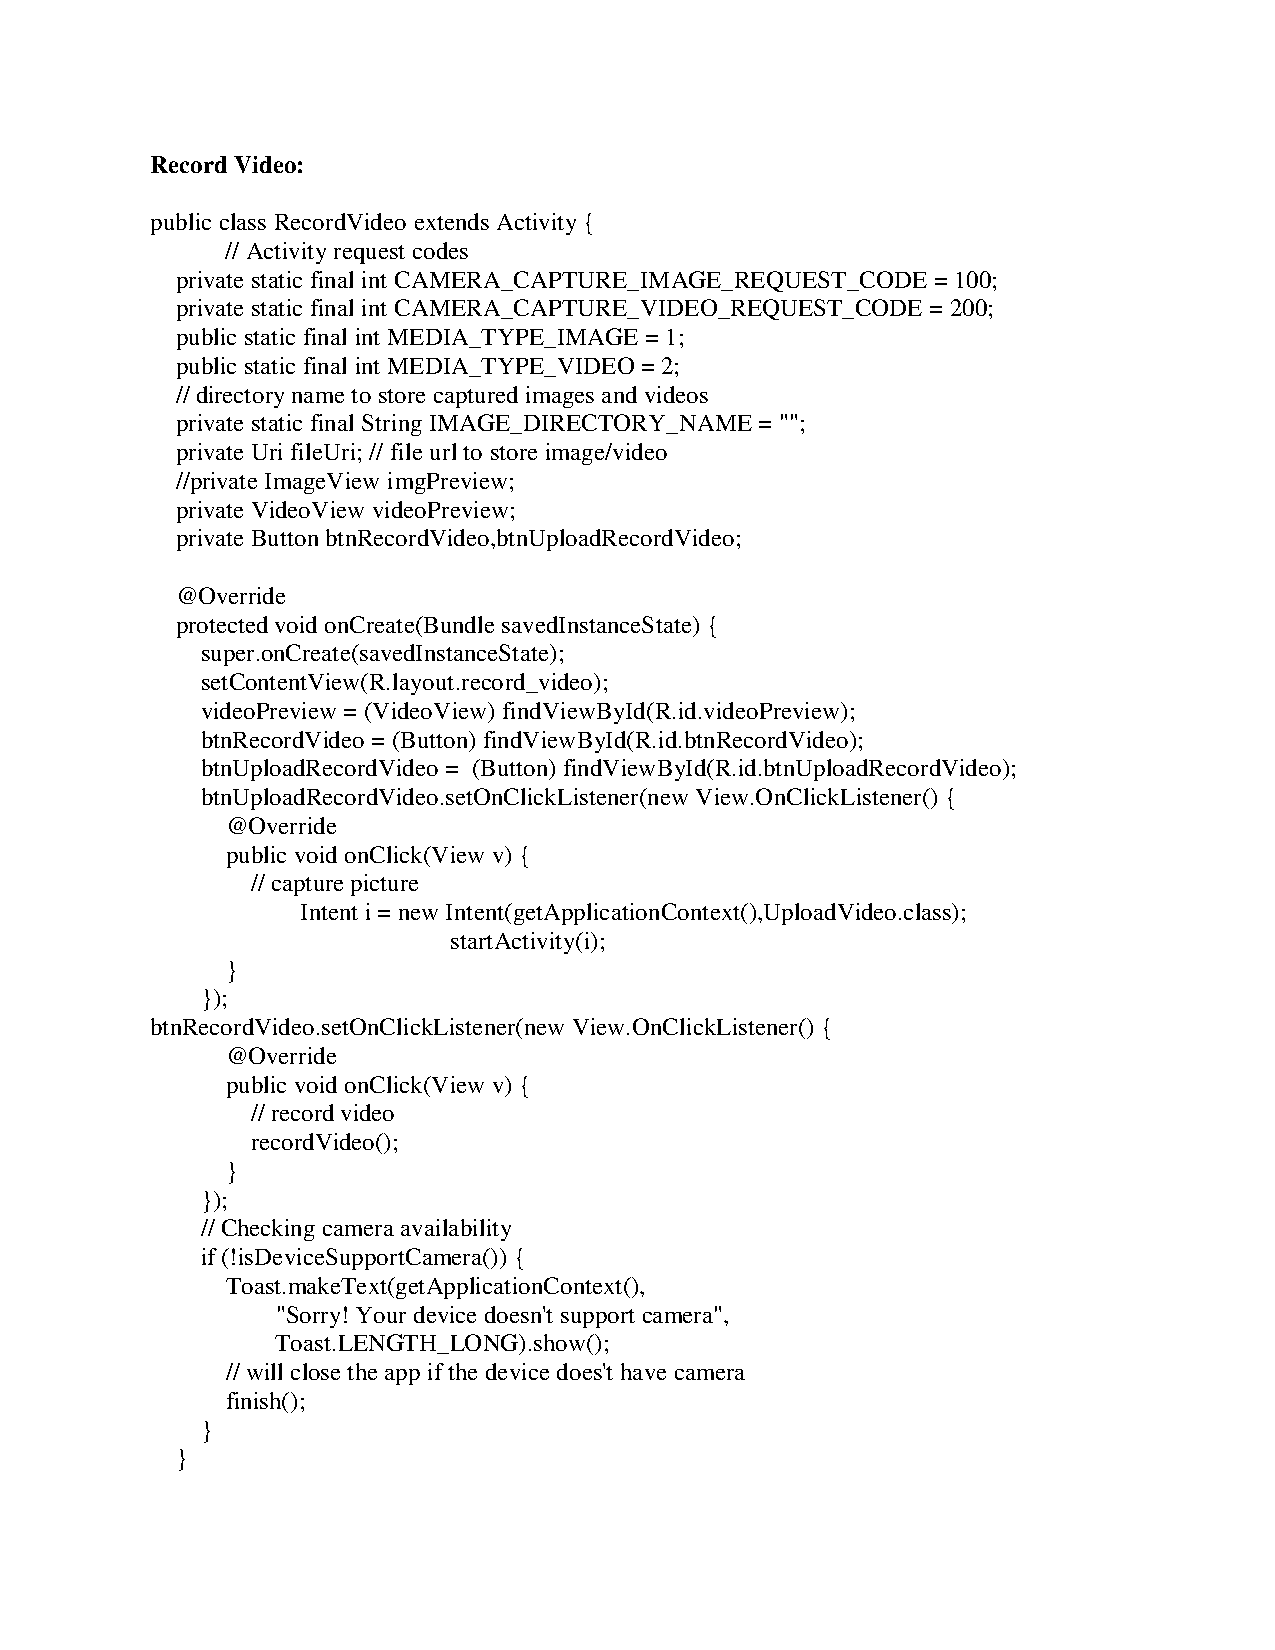
\includegraphics[width=6in]
{code13.pdf}
%\caption{snapshots}
\end{figure}

\begin{figure}[h!]
\centering
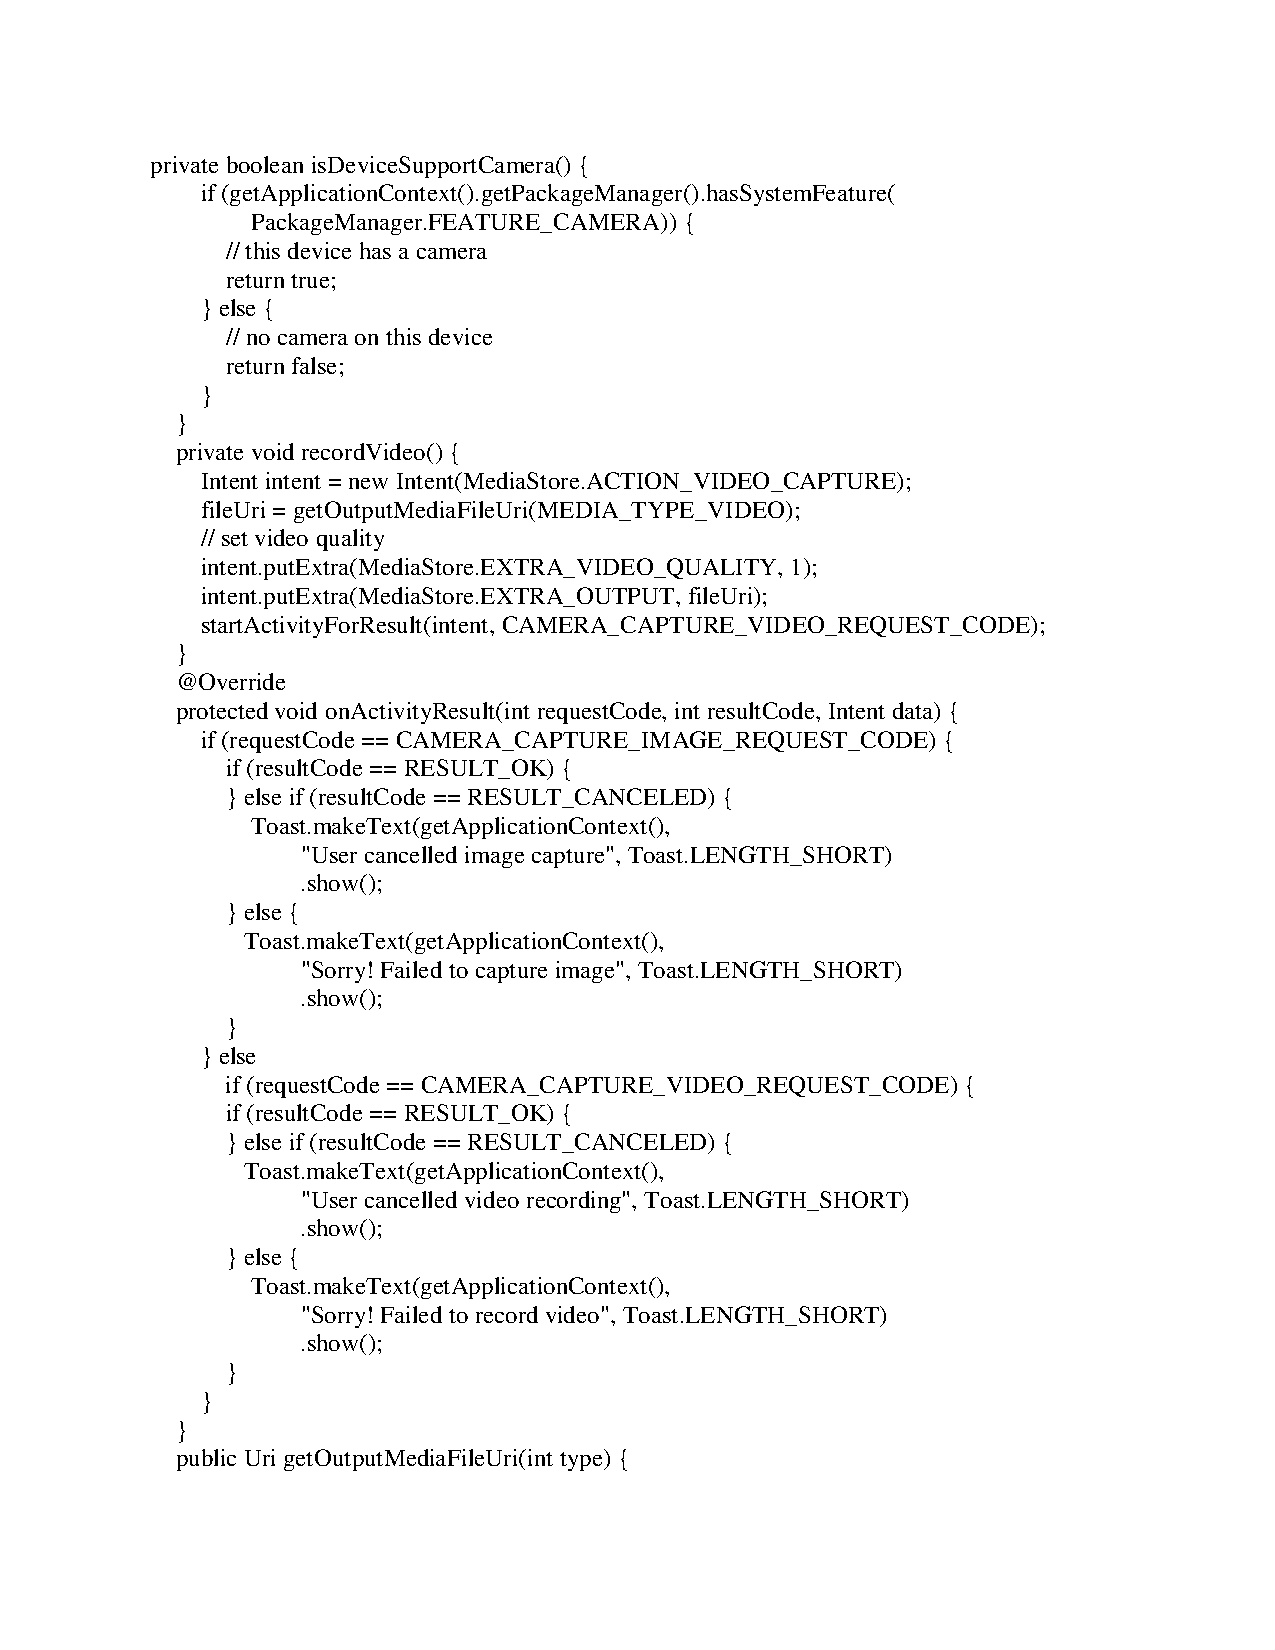
\includegraphics[width=6in]
{code14.pdf}
%\caption{snapshots}
\end{figure}

\begin{figure}[h!]
\centering
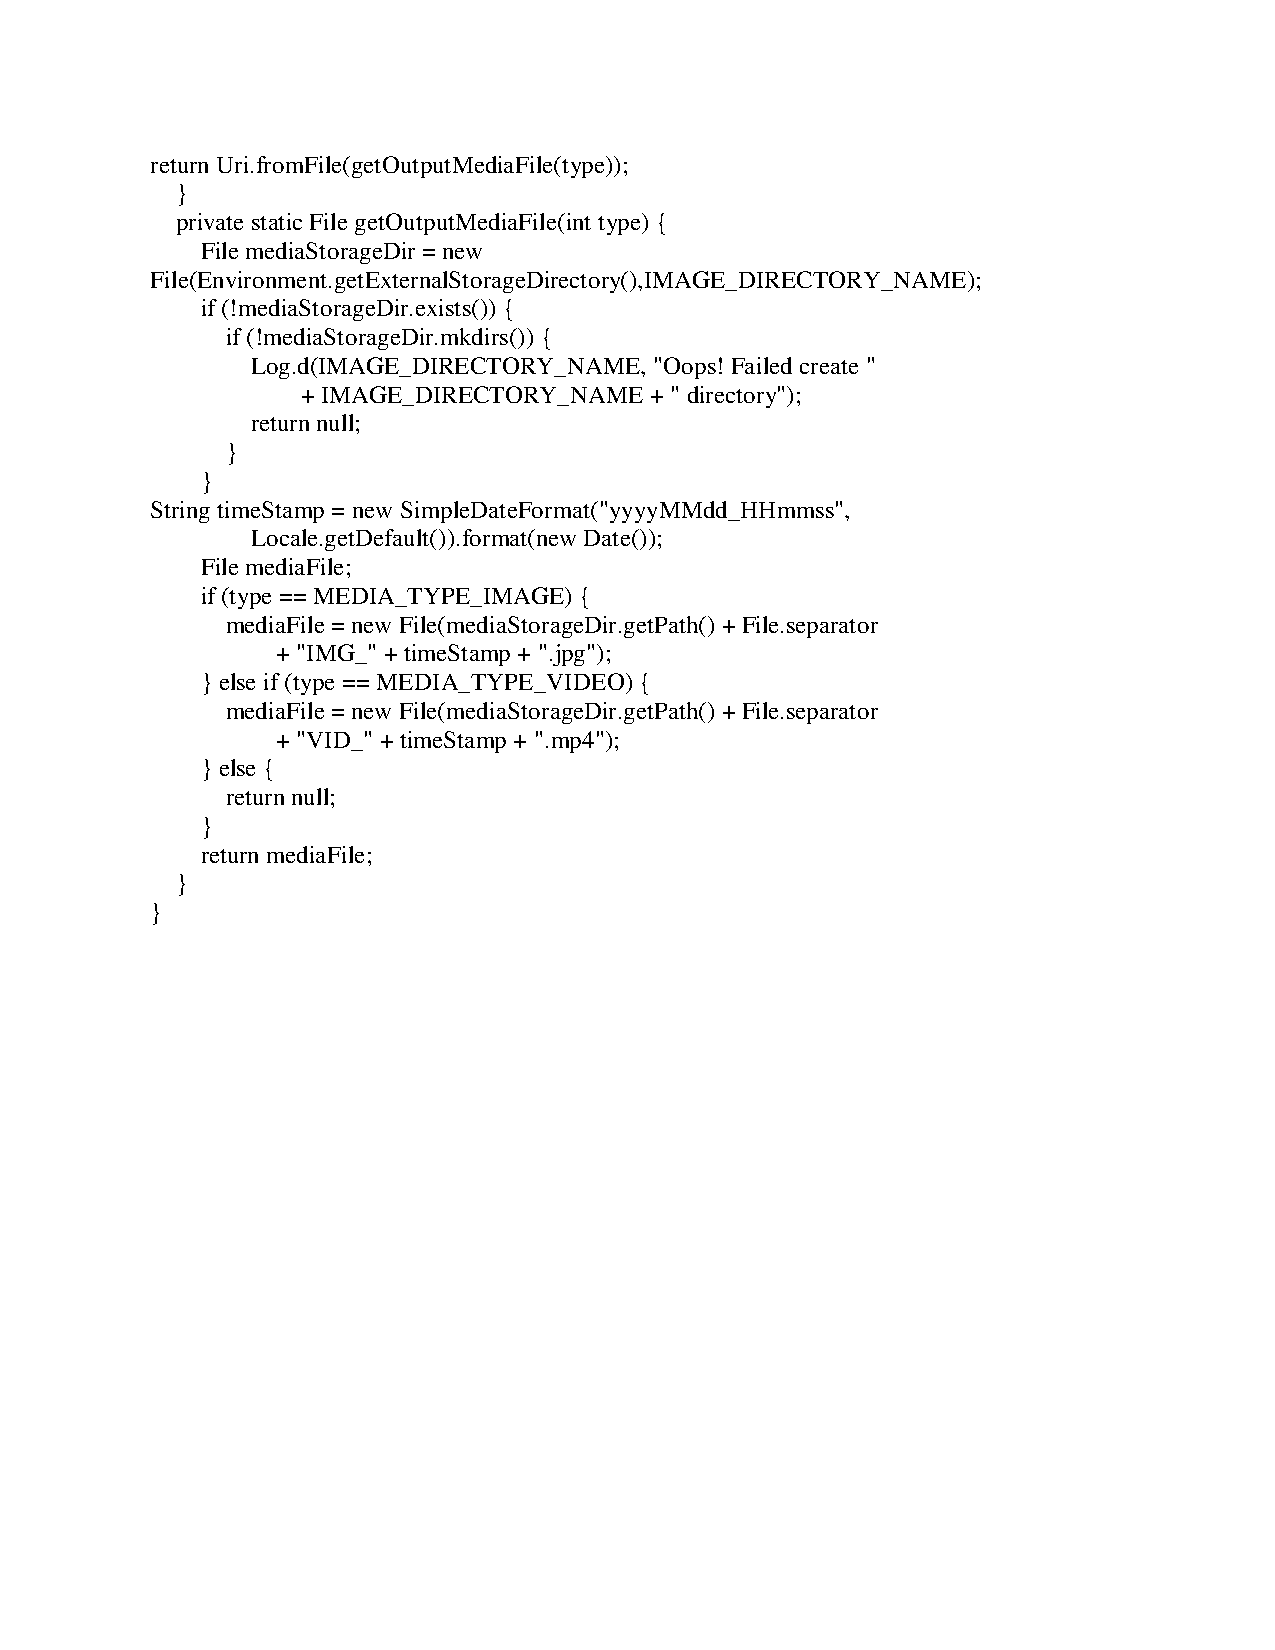
\includegraphics[width=6in]
{code15.pdf}
%\caption{snapshots}
\end{figure}